\documentclass[10pt,twoside,a4paper,fleqn]{report}

\usepackage{braket}
\usepackage{graphicx}
\usepackage{parskip}
\usepackage{amssymb}
\usepackage{mathbbol}
\usepackage{enumerate}
\usepackage{ragged2e}
\usepackage{eurosym}
\usepackage{amsmath}

% Defining some new mathematics commands
\newcommand*{\colvec}[1]{\begin{pmatrix}#1\end{pmatrix}}
\newcommand*{\0}{$\ket{0}$}
\newcommand*{\1}{$\ket{1}$}

\usepackage[english,bt]{ethidsc} % Special IDSC styles and commands      	
\usepackage{apacite}
								 % {german}/english: language of headings, etc.
								 % {st}/bt/mt: {semester}/bachelor/master thesis
							
% Page header (don't change)____________________________________________________
\setlength{\parindent}{0em}                 % Disable parindent
\rhead[\nouppercase{\rightmark}]{\thepage}  % Special headings
\lhead[\thepage]{\nouppercase{\leftmark}}   % Special headings
\cfoot{}                                    % Special headings


% Title page (please fill in)___________________________________________________
\title{Quantum Machine Learning}


\studentA{Mark Fingerhuth}
\ethidA{I6082973}
\semesterA{5}
\emailA{m.fingerhuth@student.maastrichtuniversity.nl}

%\studentB{Second Student}
%\ethidB{12-345-678}
%\semesterB{9}
%\emailB{second@student.ethz.ch}

\supervision{Prof. Francesco Petruccione\\ Dr. Fabrice Birembaut}
\date{January 2017}

\identification{IDSC-XX-YY-ZZ} 		% Project identifier

\infopage %includes the last page
\declaration

% Begin document________________________________________________________________
\begin{document}

\maketitle 							% Create title page


% Preamble______________________________________________________________________

\pagenumbering{roman} 				% Begin roman page numbering (i,ii,...)

%---------------------------------------------------------------------------
% Preface

\chapter*{Preface}

Blah blah \dots

 \cleardoublepage

%---------------------------------------------------------------------------
% Table of contents

 \setcounter{tocdepth}{2}
 \tableofcontents

 \cleardoublepage

%---------------------------------------------------------------------------
% Abstract

\chapter*{Abstract}
 \addcontentsline{toc}{chapter}{Abstract}

Blah blah \dots

 \cleardoublepage

%---------------------------------------------------------------------------
% Symbols

\chapter*{Nomenclature}\label{chap:symbole}
 \addcontentsline{toc}{chapter}{Nomenclature}

\section*{Symbols}
\begin{tabbing}
 \hspace*{1.6cm} \= \hspace*{8cm} \= \kill
 $\otimes$ \> Tensor product \\[0.5ex]
 $i$ \> Imaginary unit \> $i=\sqrt{-1}$ \\[0.5ex]
 $\dagger$ \> Hermitian conjugate \> Complex conjugate transpose \\[0.5ex]
\end{tabbing}

\section*{Indicies}
\begin{tabbing}
 \hspace*{1.6cm}  \= \kill
 a \> Ambient \\[0.5ex]
 air \> Air
\end{tabbing}

\section*{Acronyms and Abbreviations}
\begin{tabbing}
 \hspace*{1.6cm}  \= \kill
 QML \> Quantum machine learning \\[0.5ex]
 QC \> Quantum computer \\[0.5ex]
 Prob \> Probability \\[0.5ex]
 CNOT \> Controlled NOT gate \\[0.5ex]
 CCNOT \> Controlled controlled NOT gate \\[0.5ex]
 CU \> Controlled U gate (where U can be any unitary quantum gate) \\[0.5ex]
\end{tabbing}

 \cleardoublepage

%---------------------------------------------------------------------------


% Chapters______________________________________________________________________

\pagestyle{fancy}               	% Fancy headings
\pagenumbering{arabic}				% Begin arabic page numbering (1,2,...)

\chapter{Introduction}\label{sec:introduction}

\section{Quantum Bits}
\label{subsec:qubits}

INTRODUCE CONCEPT OF DROPPING GLOBAL PHASE SOMEWHERE!

\subsection{Single Qubit Systems}
\label{subsubsec:qubits}
%Classical computers manipulate bits and the quantum equivalent is called a quantum bit, often abbreviated as qubit.
Classical computers manipulate bits, whereas quantum computer's most fundamental unit is called a quantum bit, often abbreviated as qubit. Bits as well as qubits are binary entities, meaning they can only take the values 0 and 1. A classical non-probabilistic bit can only be in one of the two possible states at once. In contrast, qubits obey the laws of quantum mechanics, which gives rise to the powerful property that - besides being a definite 0 or 1 - they can also be in a superposition of the two states. Mathematically this is expressed as a linear combination of the states 0 and 1:
\begin{equation}
\label{equ: simplequbit}
\ket{\psi} = \alpha \ket{0} + \beta \ket{1}
\end{equation}
where $\alpha$ and $\beta$ are complex coefficients ($\alpha, \beta \in \mathbb{C}$) and are often referred to as phase factors or amplitudes. \0 is the Dirac notation for the qubit being in state 0 and it represents a two-dimensional vector in a complex 2-D vector space (called Hilbert space $\mathcal{H}_{2}$). \0 and \1 are the computational basis states and they constitute an orthonormal basis of $\mathcal{H}_{2}$. For the sake of clarity, \0 and \1 can be thought of as the 2-D vectors shown below.
\begin{equation}
\label{equ: 0and1kets}
\ket{0} =  \colvec{1\\0} \quad \quad \ket{1} = \colvec{0\\1}
\end{equation}

Subbing these vectors into Equ.~\ref{equ: simplequbit} yields the vector representation of $\ket{\psi}$:
\begin{equation}
\label{equ: simplequbitvector}
\ket{\psi} = \alpha \colvec{1\\0} + \beta \colvec{0\\1} = \colvec{\alpha\\\beta}
\end{equation}

However, even though a qubit can be in a superposition of \0 and \1, when measured it will take the value \0 with a probability of
\begin{equation}
\label{equ:bornrule0}
Prob(\ket{0}) = {|\alpha|}^{2}
\end{equation}
and \1 with a probability of 
\begin{equation}
\label{equ:bornrule1}
Prob(\ket{1}) = {|\beta|}^{2}
\end{equation}

The fact that the probability of measuring a particular state is equal the absolute value squared of the respective amplitude is called Born's rule (citation). Since the total probability of measuring any value has to be 1, the following normalization condition must be satisfied:
\begin{equation}
\label{equ: normalization}
{|\alpha|}^{2} + {|\beta|}^{2} =  1
\end{equation}
Therefore, a qubit is inherently probabilistic but when measured it collapses into a single classical bit (0 or 1). It follows that a measurement destroys information about the superposition of the qubit (the values of $\alpha$ and $\beta$). This constitutes one of the main difficulties when designing quantum algorithms since only limited information can be obtained about the final states of the qubits in the quantum computer.

Using spherical polar coordinates, a single qubit can be visualized on the so-called Bloch sphere by parameterising $\alpha$ and $\beta$ in Equ.~\ref{equ: simplequbit} as follows:

\begin{equation}
\label{equ: blochqubit}
\ket{q} = \cos\frac{\theta}{2} \ket{0} + e^{i \phi} \sin\frac{\theta}{2} \ket{1}
\end{equation}

The Bloch sphere has a radius of 1 and is therefore a unit sphere. The \0 qubit state is defined to lie along the positive z-axis ($\hat{z}$) and the \1 state is defined to lie along the negative z-axis ($-\hat{z}$) as labelled in Fig.~\ref{fig:blochsphere}. At this point, it is important to note that these two states are mutually orthogonal in $\mathcal{H}_{2}$ even though they are not orthogonal on the Bloch sphere. 

Qubit states on the Bloch equator such as the $\hat{x}$ and $\hat{y}$ coordinate axes represent equal superpositions where \0 and \1 both have measurement probabilities equal to $0.5$. The $\hat{x}$-axis for example represents the equal superposition $\ket{q} = \frac{1}{\sqrt{2}} \ket{0} + \frac{1}{\sqrt{2}} \ket{1}$. As illustrated in Fig.~\ref{fig:blochsphere} any arbitrary 2-D qubit state $\ket{\psi}$ can be decomposed into the polar angles $\theta$ and $\phi$ and visualized as a vector on the Bloch sphere. Such an object is called the Bloch vector of the qubit state $\ket{\psi}$. The Bloch sphere will be the main visualization tool for qubit manipulations in this thesis.

\begin{figure}[!ht]
       \centering
       \includegraphics[scale=0.07]{img/blochsphere.png}
       \caption{\label{fig:blochsphere} An arbitrary two-dimensional qubit $\ket{\psi}$ visualized on the Bloch sphere.$^{1}$}
\end{figure}

\footnotetext[1]{Reprinted from Wikipedia, n.d., Retrieved September 7, 2016, from \url{https://en.wikipedia.org/wiki/Bloch_Sphere}. Copyright 2012 by Glosser.ca. Reprinted with permission.}

\subsection{Multiple Qubit Systems}
\label{subsec:multiplequbitsystems}

Introduce tensor products here!

\subsection{Entanglement}
\label{subsec:entanglement}

Introduce entanglement and non-factorising tensor states here!

%%%%% SECTION: Q LOGIC GATES


\section{Quantum Logic Gates}
\label{subsec:quantumlogicgates}
In order to perform quantum computations, tools, analogous to the classical logic gates, are needed for qubit manipulation. Quantum logic gates are square matrices that can be visualized as rotations on the Bloch sphere. The following subsections will introduce the major single and multi qubit logic gates.

\subsection{Single Qubit Gates}
\label{subsubsec:singlequbitgates}

ADD THE CIRCUIT REPRESENTATIONS OF THE RESPECTIVE GATES!

In the following section we will evaluate the action of the most common single qubit gates on an arbitrary qubit state $\ket{\psi}$ defined in Equ.~\ref{equ: simplequbitvector}.

%The four most basic single-qubit quantum gates are given by the four Pauli matrices listed below in Equ. ~\ref{equ: paulimatrices}.

%\begin{align}
%\label{equ: paulimatrices}
%\sigma_{0} &= \mathbb{1} = \begin{pmatrix}
% 1 & 0 \\ 
% 0 & 1
% \end{pmatrix}
% \quad
% &&\sigma_{1} = \sigma_{x} = \begin{pmatrix}
% 0 & 1 \\ 
% 1 & 0
% \end{pmatrix}
% \nonumber
% \\
% \sigma_{2} &= \sigma_{y} = \begin{pmatrix}
% 0 & -i \\ 
% i & 0
% \end{pmatrix}
% \quad
% &&\sigma_{3} = \sigma_{z} = \begin{pmatrix}
% 1 & 0 \\ 
% 0 & -1
% \end{pmatrix}
%\end{align}

\subsubsection{Identity Gate}
\label{subsubsubsec:identitygate}

The simplest quantum gate is the identity or idle gate given by the 0\textsuperscript{th} Pauli matrix:

\begin{equation}
\sigma_{0} = \mathbb{1} = \begin{pmatrix}
 1 & 0 \\ 
 0 & 1
 \end{pmatrix}
\end{equation}

The action of a quantum gate on a qubit state can be analysed using the gate's matrix and the qubit's vector representation. Applying some straightforward linear algebra in this case yields:

\begin{equation}
\label{equ:identityverification}
\mathbb{1} \otimes \ket{\psi} = \mathbb{1} \otimes (\alpha \ket{0} + \beta \ket{1}) = \begin{pmatrix}
 1 & 0 \\ 
 0 & 1
 \end{pmatrix} \begin{pmatrix}
 \alpha  \\ 
 \beta
 \end{pmatrix} = \begin{pmatrix}
 \alpha  \\ 
 \beta
 \end{pmatrix} = \alpha \ket{0} + \beta \ket{1} = \ket{\psi}
\end{equation}

Hence, applying the identity gate to an arbitrary qubit state $\ket{\psi}$ leaves the state unchanged as shown in Equ.~\ref{equ:identityverification}. The idle gate is mainly used for measuring the error and lifetimes of qubits since it only evolves the qubit in time without actively rotating its Bloch vector.

\subsubsection{Qubit Flip (X) Gate}
\label{subsubsubsec:xgate}

The quantum equivalent of the classical NOT gate is called X gate and is given by the 1\textsuperscript{st} Pauli matrix:

\begin{equation}
\sigma_{1} = X = \begin{pmatrix}
 0 & 1 \\ 
 1 & 0
 \end{pmatrix}
\end{equation}

The action of the X gate is easily verified by performing some linear algebra,

\begin{equation}
\label{equ:xverification1}
X \otimes \ket{\psi} = X \otimes (\alpha \ket{0} + \beta \ket{1}) = \begin{pmatrix}
 0 & 1 \\ 
 1 & 0
 \end{pmatrix} \begin{pmatrix}
 \alpha  \\ 
 \beta
 \end{pmatrix} = \begin{pmatrix}
 \beta  \\ 
 \alpha
 \end{pmatrix} = \beta \ket{0} + \alpha \ket{1}
\end{equation}

Thus, applying the X gate to qubit state $\ket{\psi}$ swaps the amplitudes of \0 and \1. More specifically, applying X to the \0 state results in the \1 state,

\begin{equation}
\label{equ:xverification2}
X \otimes \ket{0} = \begin{pmatrix}
 0 & 1 \\ 
 1 & 0
 \end{pmatrix} \begin{pmatrix}
 1  \\ 
 0
 \end{pmatrix} = \begin{pmatrix}
 0  \\ 
 1 \end{pmatrix} =  \ket{1}
\end{equation}

And the \0 state is recovered when applying X again to the \1 state,

\begin{equation}
\label{equ:xverification3}
X \otimes \ket{1} = \begin{pmatrix}
 0 & 1 \\ 
 1 & 0
 \end{pmatrix} \begin{pmatrix}
 0  \\ 
 1
 \end{pmatrix} = \begin{pmatrix}
 1  \\ 
 0 \end{pmatrix} =  \ket{0}
\end{equation}

On the Bloch sphere, the X gate corresponds to a anti-clockwise $\pi$ rotation around the x-axis as shown in Fig.~\ref{img:blochxgate}.

\begin{figure}[ht]
   \centering
   \includegraphics[width=0.5\textwidth]{img/blochxgate.png}
   \caption{Visualization of the X gate on the Bloch sphere. Initial state (black) transformed to final state (red).}
   \label{img:blochxgate}
\end{figure}

From Equ.~\ref{equ:xverification1},~\ref{equ:xverification2} and~\ref{equ:xverification3} it follows that X is its own inverse as well as its own Hermitian conjugate:
\begin{align}
XX &= XX^\dagger = \mathbb{1} \\
X &= X^{-1} = X^\dagger
\end{align}

\subsubsection{Phase Flip (Z) Gate}
\label{subsubsubsec:zgate}

The phase flip gate, often called Z gate, is a quantum logic gate without classical equivalent. Its matrix representation is given by the 3\textsuperscript{rd} Pauli matrix:

\begin{equation}
\sigma_{3} = Z = \begin{pmatrix}
 1 & 0 \\ 
 0 & -1
 \end{pmatrix}
\end{equation}

It acts on $\ket{\psi}$ as follows:

\begin{equation}
\label{equ:zverification1}
Z \otimes \ket{\psi} = Z \otimes (\alpha \ket{0} + \beta \ket{1}) = \begin{pmatrix}
 1 & 0 \\ 
 0 & -1
 \end{pmatrix} \begin{pmatrix}
 \alpha  \\ 
 \beta
 \end{pmatrix} = \begin{pmatrix}
 \alpha  \\ 
 -\beta
 \end{pmatrix} = \alpha \ket{0} - \beta \ket{1}
\end{equation}

Applying Z again recovers the initial state,

\begin{equation}
\label{equ:zverification2}
Z \otimes (\alpha \ket{0} - \beta \ket{1}) = \alpha \ket{0} + \beta \ket{1} = \ket{\psi}
\end{equation}

Fig.~\ref{img:blochzgate} visualizes that the Z gate corresponds to a anti-clockwise $\pi$ rotation around the z-axis.

\begin{figure}[ht]
   \centering
   \includegraphics[width=0.5\textwidth]{img/blochzgate.png}
   \caption{Visualization of the Z gate on the Bloch sphere. Initial state (black) transformed to final state (red).}
   \label{img:blochzgate}
\end{figure}

From Equ.~\ref{equ:zverification1} and Equ.~\ref{equ:zverification2}, it follows that also Z is its own inverse as well as Hermitian conjugate:
\begin{align}
ZZ &= ZZ^\dagger = \mathbb{1} \\
Z &= Z^{-1} = Z^\dagger
\end{align}

\subsubsection{Qubit and Phase Flip (Y) Gate}
\label{subsubsubsec:ygate}

The combined qubit and phase flip gate, also called Y gate, is a quantum logic gate without classical equivalent since it involves the complex number i ($\sqrt{-1}$). Its matrix representation is given by the 2\textsuperscript{nd} Pauli matrix:

\begin{equation}
\sigma_{2} = Y = \begin{pmatrix}
 0 & -i \\ 
 i & 0
 \end{pmatrix}
\end{equation}

It essentially combines the action of the X and the Z gate since it exchanges the amplitudes and adds a phase to the qubit state:

\begin{equation}
\label{equ:yverification1}
Y \otimes \ket{\psi} = Y \otimes (\alpha \ket{0} + \beta \ket{1}) = \begin{pmatrix}
 0 & -i \\ 
 i & 0
 \end{pmatrix} \begin{pmatrix}
 \alpha  \\ 
 \beta
 \end{pmatrix} = \begin{pmatrix}
 -i\beta  \\ 
 i\alpha
 \end{pmatrix} = -i\beta \ket{0} + i\alpha \ket{1}
\end{equation}

One can simplify the last expression since a so-called global phase of $i$ is present which can be factored out:

\begin{equation}
\label{equ:yverification2}
-i\beta \ket{0} + i\alpha \ket{1} = i(-\beta \ket{0} + \alpha \ket{1}) = -\beta \ket{0} + \alpha \ket{1}
\end{equation}

To proof this, one calculates the probability of measuring the \0 state including the global phase (last expression in Equ.~\ref{equ:yverification1}) by taking the absolute value squared of the amplitude of the \0 state:

\begin{equation}
\label{equ:globalphase}
Prob(\ket{0}) = \mid-i\beta\mid^2 = (-i\beta)(i\beta) = -i^2\beta^2 = -(\sqrt{-1})^2\beta^2 = \beta^2
\end{equation}

When calculating the probability whilst omitting the global phase of $i$ one arrives at the same result: 

\begin{equation}
\label{equ:globalphase}
Prob(\ket{0}) = \mid-\beta\mid^2 = \beta^2
\end{equation}

It follows that a global phase is immeasurable in experiments and can therefore be left out.

The Y gate corresponds to a $\pi$ rotation around the y-axis of the Bloch sphere as shown in Fig.~\ref{img:blochygate}.

\begin{figure}[ht]
   \centering
   \includegraphics[width=0.5\textwidth]{img/blochygate.png}
   \caption{Visualization of the Y gate on the Bloch sphere. Initial state (black) transformed to final state (red).}
   \label{img:blochygate}
\end{figure}

From Equ.~\ref{equ:yverification1} it follows that, similar to the X and Z gate, the Y gate is its own inverse and Hermitian conjugate:

\begin{align}
YY &= YY^\dagger = \mathbb{1} \\
Y &= Y^{-1} = Y^\dagger
\end{align}


\subsubsection{Hadamard (H) Gate}
\label{subsubsubsec:hadamardgate}

In order to create superpositions from an initial \0 or \1 state the Hadamard or H gate is required. It is defined by the following matrix:

\begin{equation}
H = \begin{pmatrix}
 \frac{1}{\sqrt{2}} & \frac{1}{\sqrt{2}} \\ 
 \frac{1}{\sqrt{2}} & -\frac{1}{\sqrt{2}}
 \end{pmatrix}
\end{equation}

The action of the H gate is best understood when applying it to the \0 state,

\begin{equation}
\label{equ:hadamardverification1}
H \otimes \ket{0} = \begin{pmatrix}
 \frac{1}{\sqrt{2}} & \frac{1}{\sqrt{2}} \\ 
 \frac{1}{\sqrt{2}} & -\frac{1}{\sqrt{2}}
 \end{pmatrix} \begin{pmatrix}
 1 \\ 
 0
 \end{pmatrix} = \begin{pmatrix}
 \frac{1}{\sqrt{2}} \\ 
 \frac{1}{\sqrt{2}}
 \end{pmatrix} = \frac{1}{\sqrt{2}} \ket{0} + \frac{1}{\sqrt{2}} \ket{1}
\end{equation}

Thus, the H gate has transformed the \0 state into an equal superposition of \0 and \1. Similarly applying the H gate to the \1 state creates an equal superposition of \0 and \1 with an additional negative sign on the \1 state:

\begin{equation}
\label{equ:hadamardverification2}
H \otimes \ket{1} = \begin{pmatrix}
 \frac{1}{\sqrt{2}} & \frac{1}{\sqrt{2}} \\ 
 \frac{1}{\sqrt{2}} & -\frac{1}{\sqrt{2}}
 \end{pmatrix} \begin{pmatrix}
 0 \\ 
 1
 \end{pmatrix} = \begin{pmatrix}
 \frac{1}{\sqrt{2}} \\ 
 -\frac{1}{\sqrt{2}}
 \end{pmatrix} = \frac{1}{\sqrt{2}} \ket{0} - \frac{1}{\sqrt{2}} \ket{1}
\end{equation}

Fig.~\ref{img:blochhgate} illustrates how the H gate first rotates the qubit around the y-axis by $\frac{\pi}{2}$ radians followed by a $\pi$ rotation around the x-axis.

\begin{figure}[ht]
   \centering
   \includegraphics[width=0.8\textwidth]{img/blochhadamardnielsenchuang.png}
   \caption{Visualization of the Hadamard gate on the Bloch sphere, acting on the input state $\ket{q} = \frac{1}{\sqrt{2}} \ket{0} + \frac{1}{\sqrt{2}} \ket{1}$.\textsuperscript{2}}
   \label{img:blochhgate}
\end{figure}

\footnotetext[2]{Reprinted from Michael A. Nielsen and Isaac L. Chuang. Quantum Computation and Quantum Information. Cambridge University Press, 2000. Copyright 2010 by Nielsen \& Chuang.}

%\begin{figure}[ht]
%   \centering
%   \includegraphics[width=0.5\textwidth]{img/blochhadamard.png}
%   \caption{Visualization of the H gate on the Bloch sphere. Initial state (black) transformed to final state (red).}
%   \label{img:blochhgate}
%\end{figure}

Omitting the proof, from Equ.~\ref{equ:hadamardverification1} and Equ.~\ref{equ:hadamardverification2} one can easily see that the H gate is a Hermitian matrix which means it is its own Hermitian conjugate and inverse:

\begin{align}
HH &= HH^\dagger = \mathbb{1} \\
H &= H^{-1} = H^\dagger
\end{align}

\subsubsection{$\frac{\pi}{2}$ Rotation (S,S$^\dagger$) Gates}
\label{subsubsubsec:cliffordgates}

The S and S$^\dagger$ gates make it possible to reach more points on the Bloch sphere since they introduce $\frac{\pi}{2}$ rotations around the z-axis. The S gate is defined to be the square root of the Z gate and it is not Hermitian giving rise to the following two matrices: 

\begin{equation}
S = \sqrt{Z} = \begin{pmatrix}
 1 & 0 \\ 
 0 & i
 \end{pmatrix}
 \quad \quad \quad \quad
S^\dagger = \begin{pmatrix}
 1 & 0 \\ 
 0 & -i
 \end{pmatrix}
\end{equation}

The S gate simply adds an imaginary phase to the \1 state,

\begin{equation}
\label{equ:sverification}
S \otimes \ket{\psi} = S \otimes (\alpha \ket{0} + \beta \ket{1}) = \begin{pmatrix}
 1 & 0 \\ 
 0 & i
 \end{pmatrix} \begin{pmatrix}
 \alpha  \\ 
 \beta
 \end{pmatrix} = \begin{pmatrix}
 \alpha  \\ 
 i\beta
 \end{pmatrix} = \alpha \ket{0} + i\beta \ket{1}
\end{equation}

Visually this corresponds to a $\frac{\pi}{2}$ rotation around the z-axis as shown in Fig.~\ref{img:blochsgate}. In contrast, the S$^\dagger$ gate performs the inverse action and therefore rotates the qubit by $-\frac{\pi}{2}$ radians around the z-axis.

\begin{figure}[ht]
   \centering
   \includegraphics[width=0.5\textwidth]{img/blochsgate.png}
   \caption{Visualization of the S gate on the Bloch sphere. Initial state (black) transformed to final state (red).}
   \label{img:blochsgate}
\end{figure}

In contrast to all previously introduced gates, the S gate is not its own inverse or Hermitian conjugate. However, applying the S gate four times yields the identity matrix since it corresponds to a $2\pi$ rotation around the z-axis,

\begin{equation}
SSSS = \mathbb{1} = SS^\dagger
\end{equation}

\subsubsection{$\frac{\pi}{4}$ Rotation (T,T$^\dagger$) Gates}
\label{subsubsubsec:noncliffordgates}

Until this point, all introduced single qubit gates are part of the so-called Clifford group. The Gottesmann-Knill theorem states that all quantum circuits consisting only of Clifford gates can be efficiently simulated on a classical computer (citation!). To harness the full potential of quantum computation, one needs to add a non-Clifford gate to the quantum gate set. The T and T$^\dagger$ gates are such non-Clifford gates and are defined as follows,

\begin{equation}
T = \sqrt{S} = \begin{pmatrix}
 1 & 0 \\ 
 0 & e^{\frac{i\pi}{4}}
 \end{pmatrix}
\quad \quad \quad \quad
T^\dagger = \begin{pmatrix}
 1 & 0 \\ 
 0 & e^{-\frac{i\pi}{4}}
 \end{pmatrix}
\end{equation}

On the Bloch sphere, the T gate corresponds to a $\frac{\pi}{4}$ rotation around the z-axis as it can be seen in Fig.~\ref{img:blochtgate}. Consequently, the T$^\dagger$ gate constitutes a $-\frac{\pi}{4}$ rotation around the z-axis.

\begin{figure}[ht]
   \centering
   \includegraphics[width=0.5\textwidth]{img/blochtgate.png}
   \caption{Visualization of the T gate on the Bloch sphere. Initial state (black) transformed to final state (red).}
   \label{img:blochtgate}
\end{figure}

Similar to the S gate, applying the T gate eight times yields the identity matrix since eight $\frac{\pi}{4}$ rotations make a full $2\pi$ z-rotation.

\begin{equation}
TTTTTTTT = \mathbb{1} = TT^\dagger
\end{equation}

%%%%% SUBSECTION: MULTIPLE Q LOGIC GATES


\subsection{Multiple Qubit Gates}
\label{subsubsec:multiqubitgates}

\subsubsection{Controlled NOT Gate}
\label{subsubsubsec:cnotgate}

The most important two-qubit quantum gate is the controlled NOT or CNOT gate given by the following 4x4 matrix:
\begin{equation}
CNOT = \begin{pmatrix}
 \mathbb{1} & 0 \\ 
 0 & X
 \end{pmatrix} = \begin{pmatrix}
 1 & 0 & 0 & 0 \\ 
 0 & 1 & 0 & 0 \\
 0 & 0 & 0 & 1 \\
 0 & 0 & 1 & 0 \\
 \end{pmatrix}
\end{equation}

The CNOT gate takes two qubits, control and target qubit, as input. If and only if the control qubit is in the \1 state, the NOT (X) gate is applied to the target qubit. In equations, the CNOT will always be followed by parantheses containing the control qubit followed by the target qubit (e.g. CNOT(0,1)). The input-output relation for the CNOT gate is given in Table~\ref{tab:cnottruthtable} below.

\begin{table}[ht!]
\begin{center}
\caption{CNOT truth table with first qubit as control, second qubit as target.}\vspace{1ex}
\label{tab:cnottruthtable}
\begin{tabular}{llccc}\hline
Input & Output \\ \hline
00 & 00 \\
01 & 01 \\
10 & 11 \\
11 & 10 \\ \hline
\end{tabular}
\end{center}
\end{table}

To demonstrate the usefulness of the CNOT gate consider starting with two unentangled qubits both in the \0 state,

\begin{equation}
\ket{\phi} = \ket{0} \otimes \ket{0} = \ket{00}
\end{equation}

Applying the H gate onto the first qubit yields the following (still unentangled) state:

\begin{equation}
(H \otimes \mathbb{1}) \ket{\phi} = (H \otimes \mathbb{1}) \ket{00} = \frac{1}{\sqrt{2}} \ket{00} + \frac{1}{\sqrt{2}} \ket{10} 
\end{equation}

Now consider applying the CNOT to this state whereby the control qubit is coloured \textcolor{red}{red} and the target qubit \textcolor{green}{green}.

\begin{equation}
\label{equ:cnotexamples}
CNOT(\textcolor{red}{0},\textcolor{green}{1}) \otimes (\frac{1}{\sqrt{2}} \ket{\textcolor{red}{0}\textcolor{green}{0}} + \frac{1}{\sqrt{2}} \ket{\textcolor{red}{1}\textcolor{green}{0}}) = \frac{1}{\sqrt{2}} \ket{\textcolor{red}{0}\textcolor{green}{0}} + \frac{1}{\sqrt{2}} (\mathbb{1} \otimes X) \ket{\textcolor{red}{1}\textcolor{green}{0}} = \frac{1}{\sqrt{2}} \ket{\textcolor{red}{0}\textcolor{green}{0}} + \frac{1}{\sqrt{2}} \ket{\textcolor{red}{1}\textcolor{green}{1}}
\end{equation}

The last expression in Equ.~\ref{equ:cnotexamples} is one of the famous Bell states which are maximally entangled states. Thus, this example demonstrates how the CNOT gate is crucial for the generation of entangled states since it applies the X gate dependending on the state of a second qubit.

\subsubsection{Toffoli Gate}
\label{subsubsubsec:toffoligate}

Of course one can create a controlled controlled NOT (CCNOT) quantum gate which is often referred to as the Toffoli gate. It is defined by the following 8x8 matrix:
\begin{equation}
Toffoli = CCNOT = \begin{pmatrix}
 \mathbb{1}_6 & 0 \\ 
 0 & X
 \end{pmatrix} = \begin{pmatrix}
 1 & 0 & 0 & 0 & 0 & 0 & 0 & 0 \\ 
 0 & 1 & 0 & 0 & 0 & 0 & 0 & 0 \\ 
 0 & 0 & 1 & 0 & 0 & 0 & 0 & 0 \\ 
 0 & 0 & 0 & 1 & 0 & 0 & 0 & 0 \\ 
 0 & 0 & 0 & 0 & 1 & 0 & 0 & 0 \\ 
 0 & 0 & 0 & 0 & 0 & 1 & 0 & 0 \\
 0 & 0 & 0 & 0 & 0 & 0 & 0 & 1 \\ 
 0 & 0 & 0 & 0 & 0 & 0 & 1 & 0 \\ 
 \end{pmatrix}
\end{equation}

where $\mathbb{1}_6$ is the 6x6 identity matrix.

The Toffoli gate takes three inputs specified in parantheses, first the two control qubits and lastly the target qubit.

TRUTH TABLE???

\subsubsection{n-CNOT Gate}
\label{subsubsubsec:ncnotgate}
\begin{equation}
nCNOT = \begin{pmatrix}
 \mathbb{1}_{2^n-2} & 0 \\ 
 0 & X
 \end{pmatrix}
\end{equation}

\subsubsection{Controlled U Gate}
\label{subsubsubsec:controlledugate}

\begin{equation}
CU = \begin{pmatrix}
 \mathbb{1} & 0 \\ 
 0 & U
 \end{pmatrix}
\end{equation}

%%%%% SECTION: MEASUREMENTS

\section{Qubit Measurements}
\label{subsec:qubitmeasurements}

\subsection{Standard Basis Measurement}
\label{subsubsec:standardbasismeasurement}

\subsection{Bloch Measurement (?)}
\label{subsubsec:blochmeasurement}

%%%%% SECTION: MACHINE LEARNING

%\section{Machine Learning}
%\label{subsec:machinelearning}

\section{Classical Machine Learning}
\label{subsec:classicalmachinelearning}

\subsection{k-nearest Neighbour Algorithm}
\label{subsubsec:knearestneighbour}

\section{Quantum Machine Learning}
\label{subsec:quantummachinelearning}

\subsection{Quantum k-nearest Neighbour Algorithm}
\label{subsubsec:quantumknearestneighbour}

\section{Research Question}
\label{subsec:researchquestion}
\cleardoublepage
\chapter{Materials and Methods}\label{sec:materialsandmethods}
\cleardoublepage
\chapter{Results and Discussion}\label{sec:resultsanddiscussion}

Some more general text
Why are some parts simulating and some parts using IBM?
All the code can be found on GitHub\textsuperscript[7]

\footnotetext[7]{Link to GitHub folder.}

\section{Simulating the qubit-based kNN algorithm}
\label{subsec:qubitKNNresults}

The computer used for the Liqui$\ket{}$ quantum simulations in this thesis only provides 8GB of RAM, thereby limiting the maximum number of simulated qubits to 24. Unfortunately, real-world machine learning problems usually involve large datasets that would require much more qubits such that a small artificial dataset needs to be constructed. For this reason, the classification of 9-bit, little-endian RGB colour codes into the classes \emph{red} and \emph{blue} will be considered. A 9-bit RGB colour code uses three bits to encode the content of each RGB colour; red, green and blue. Three binary bits $b_0,b_1,b_2$ can encode any of the numbers 0-7 according to the formula,

\begin{equation}
b_0*2^0 + b_1*2^1 + b_2*2^2 \text{ where } b_0,b_1,b_2 \in \left\{0,1\right\}
\end{equation}

For example, the 9-bit RGB code 111 100 100 can be written in roman numerals as 7,1,1 (full red, little green, little blue) and represents \colorbox{examplered}{this red tone}.

Since the class qubit $\ket{c}$ can only take binary values, class red is defined as $\ket{c} = \ket{0}$ and class blue is defined as $\ket{c} = \ket{1}$. The training set consists of 3 randomly chosen red and blue tones listed in Table~\ref{tab:trainingcolours}.

\begin{table}
\label{tab:trainingcolours}
\centering
    \begin{tabular}{| c| c |c |}
      %\toprule
      Colour & Binary 9-bit RGB string & Class\\
      \midrule
       \cellcolor{red1} & 111 000 000 & red ($\ket{0}$)\\\midrule
       \cellcolor{red2} & 101 000 000 & red ($\ket{0}$)\\\midrule
       \cellcolor{red3} & 110 000 000 & red ($\ket{0}$)\\\midrule
       \cellcolor{blue1} & 000 000 111 & blue ($\ket{1}$)\\\midrule
       \cellcolor{blue2} & 000 000 101 & blue ($\ket{1}$)\\\midrule
       \cellcolor{blue3} & 000 000 100 & blue ($\ket{1}$)\\\midrule
      \bottomrule
    \end{tabular}
    \caption{Training data set of six 9-bit RGB colour codes}
\end{table}

The quantum classifier will then be tested on four new colour tones (two red, two blue) listed in Table~\ref{tab:inputcolours}. Note that all training colours are either pure red colours (without green or blue content) or pure blue colours (without green or red content). The input colours, however, also include colours with additional green content testing how the classifier reacts in cases that are not included in the training set.

\begin{table}
\centering
    \begin{tabular}{| c| c |c |}
      %\toprule
      Colour & Binary 9-bit RGB string & Expected classification outcome\\
      \midrule
       \cellcolor{inputred1} & 100 000 000 & red ($\ket{0}$)\\\midrule
              \cellcolor{inputmixred2} & 110 100 000 & red ($\ket{0}$)\\\midrule

       \cellcolor{inputblue1} & 000 000 110 & blue ($\ket{1}$)\\\midrule
       \cellcolor{inputmixblue2} & 000 100 111 & blue ($\ket{1}$)\\\midrule
      \bottomrule
    \end{tabular}
    \label{tab:inputcolours}
    \caption{Input data set containing 9-bit RGB colour codes that require classification}
\end{table}

The first step towards the classification of RGB colour codes using the qubit-based kNN algorithm proposed by \citeA{Schuld2014} as described in detail in Section~\ref{subsubsec:quantumknearestneighbour} is preparing the initial superposition over all six 9-bit RGB training patterns $t^j$:

\begin{equation}
\label{equ:trainingsup}
\ket{T} = \frac{1}{\sqrt{6}}\sum_{j=1}^N \ket{t_1^j,t_2^j,...t_9^j;c^j}
\end{equation}

This can be done using the quantum state preparation algorithm by \citeA{Trugenberger2001} outlined in Section~\ref{subsubsec:classicaldataqubits}. In this case, the seven steps (see blue box in Section~\ref{subsubsec:classicaldataqubits}) of the state preparation algorithm have to be repeated six times in order to load the six RGB training patterns $t^j$ into the memory register $m$ defined in Equ.~\ref{equ:truginitial}. Afterwards, the state is given by,

\begin{equation}
\label{equ:trugcolours}
\ket{\phi_0} = \frac{1}{\sqrt{6}} \sum^6_{j=1} \ket{t^6_1,t^6_2,...,t^6_9;u_1=0,u_2=0;t^j_1,t^j_2,...,t^j_9}
\end{equation}

Equ.~\ref{equ:trugcolours} shows that the first register still contains the last stored RGB colour code $t^6$, the second register consists of the utility qubits $\ket{u_1}$ and $\ket{u_2}$ that are both in the \0 state and the last register is in an equal superposition over all six RGB training colours. Thus, besides the missing class qubit $\ket{c}$ the last register is in the desired superposition defined in Equ.~\ref{equ:trainingsup}.

In the next step of the quantum kNN the yet unclassified 9-bit RGB input pattern $x$ and an ancilla qubit $\ket{a}$ initialized in state \0 are added to the training superposition $\ket{T}$ to result in the full initial state $\ket{\psi_0}$:

\begin{equation}
\label{equ:fullinitialstate}
\ket{\psi_0} = \frac{1}{\sqrt{6}}\sum_{j=1}^6 \ket{x_1,x_2,...x_9;t_1^j,t_2^j,...t_9^j;c^j;0}
\end{equation}

The trick now is to realize that Equ.~\ref{equ:trugcolours} and ~\ref{equ:fullinitialstate} contain the same number of qubits. Firstly, each of them has nine qubits in the first register. Secondly, Equ.~\ref{equ:trugcolours} has two utility qubits that are balanced by the ancilla and the class qubit in Equ.~\ref{equ:fullinitialstate}. Lastly, there are again nine qubits in the third register in Equ.~\ref{equ:trugcolours} and the second register in Equ.~\ref{equ:fullinitialstate}. Thus, $\ket{\psi_0}$ and $\ket{\phi}$ both contain $9+9+2 = 20$ qubits. Since $\ket{\phi}$ is the current state of the qubits in the simulation, one simply needs to redefine the utility qubits such that the first one becomes the class qubit $\ket{u_1} = \ket{c^j}$ and the second utility qubit becomes the ancilla $\ket{u_2} = \ket{a}$. Note that class and ancilla qubit are currently still in the \0 state as indicated in the current quantum state $\ket{\phi_1}$:

\begin{equation}
\label{equ:trugcolours2}
\ket{\phi_1} = \frac{1}{\sqrt{6}} \sum^6_{j=1} \ket{t^6_1,t^6_2,...,t^6_9;c^j=0;a=0;t^j_1,t^j_2,...,t^j_9}
\end{equation}

Equ.~\ref{equ:trugcolours2} shows a quantum state with four registers as desired but the first register still contains the last training colour code $t^6$. However, it can simply be overwritten with the desired input pattern by comparing the two patterns and flipping qubits at positions where the patterns do not match up. For example, if the last training pattern was 000 000 100 and the input pattern is 000 000 110 one simply needs to flip the 8\textsuperscript{th} qubit through the application of an X gate. The state is now given by,

\begin{equation}
\label{equ:trugcolours3}
\ket{\phi_2} = \frac{1}{\sqrt{6}} \sum^6_{j=1} \ket{x_1,x_2,...,x_9;c^j=0;a=0;t^j_1,t^j_2,...,t^j_9}
\end{equation}

Currently, every training pattern is considered class $\ket{0}$ (red) which is of course incorrect. To flip the class qubit for the three training patterns encoding blue colours, one can make use of X and nCNOT gates. Consider the fourth (first blue) training pattern $t^4$ = 000 000 111 from Table~\ref{table:trainingcolours}. One might think that simply applying a 3CNOT($t_7,t_8,t_9$,c) gate controlled by the three qubits that are in the \1 state will suffice to flip the class label for this training pattern. However, depending on the classification problem at hand there might be another training pattern e.g. $t'$ = 111 110 111 belonging to class \0 for which the application of the 3CNOT($t_7,t_8,t_9$,c) gate would incorrectly flip the class qubit since the last three qubits of $t'$ are also in the \1 state.

To avoid this problem, apply an X gate to all qubits in the training pattern that are currently in the \0 state. Continuing the example with the training pattern $t^4$ = 000 000 111, X gates need to be applied to the first six qubits. The result is then $t^{4*}$ = 111 111 111. After this step, any other training pattern will contain at least one zero e.g. flipping the first six qubits of $t'$ = 111 110 111 results in $t'^{*}$ = 000 001 111. Hence, the training pattern $t^4$ is now the only pattern in the fourth register consisting only of ones. Now, this property can be exploited by applying a 9CNOT($t_1,t_2,...,t_9$,c) gate that will flip the class label to $\ket{1}$ for training pattern $t^4$ only. Acting X gates on the first six qubits again will restore all training patterns to their original states. Repeating this procedure for all training patterns belonging to class $\ket{1}$ (blue) entangles the class qubit $\ket{c}$ with the training patterns and the overall state is now described by,

\begin{equation}
\label{equ:trugcolours4}
\ket{\phi_3} = \frac{1}{\sqrt{6}} \sum^6_{j=1} \ket{x_1,x_2,...,x_9;c^j;a=0;t^j_1,t^j_2,...,t^j_9}
\end{equation}

Note that the class qubit is now not in the \0 state only. Inspection of Equ.~\ref{equ:trugcolours4} reveals that $\ket{\phi_3}$ is identical to the desired initial state $\ket{\psi_0}$ defined in Equ.~\ref{equ:fullinitialstate} the only difference being the position of the class and ancilla register. One can now proceed with the quantum kNN routine by simply putting the ancilla register into superposition with an H gate.

\begin{equation}
\label{equ:trugcolours5}
\ket{\phi_4} = \frac{1}{\sqrt{12}} \sum^6_{j=1} \Big[\ket{x_1,x_2,...,x_9;c^j;0;t^j_1,t^j_2,...,t^j_9} + \ket{x_1,x_2,...,x_9;c^j;1;t^j_1,t^j_2,...,t^j_9}\Big]
\end{equation}

The next step is the calculation of the HD between the input pattern and each training pattern which is done by the straightforward application of nine CNOT($x_s,t_s^j$) gates. By applying an X gate to every qubit in the fourth register the HD gets reversed as discussed in Section~\ref{subsubsec:quantumknearestneighbour}. The state is now,


\begin{align}
\ket{\phi_5} = \frac{1}{\sqrt{12}} \sum^6_{j=1} \prod_{s=1}^9 X(t^j_s)CNOT(x_s,t^j_s) \Big[&\ket{x_1,x_2,...,x_9;c^j;0;t^j_1,t^j_2,...,t^j_9}\notag\\
&+ \ket{x_1,x_2,...,x_9;c^j;1;t^j_1,t^j_2,...,t^j_9}\Big]
\end{align}
\begin{equation}
\quad\quad = \frac{1}{\sqrt{12}} \sum^6_{j=1} \Big[\ket{x_1,x_2,...,x_9;c^j;0;d_1^j,d_2^j,...d_9^j} + \ket{x_1,x_2,...,x_9;c^j;1;d_1^j,d_2^j,...d_9^j}\Big]
\end{equation}


In order to perform the sum over the fourth register and store the result in the complex phase of the corresponding term in the superposition one needs to implement the unitary operator $U$ previously defined in Equ.~\ref{equ:sumoperator} and \ref{equ:sumoperator2} with $n = 9$ in the case of 9-bit RGB classification. According to \citeA{Trugenberger2001} the operator $U$ can be decomposed as follows:

\begin{align}
&U\ket{\phi_5} = e^{-i\frac{\pi}{2n}K}\ket{\phi_5} = e^{-i\frac{\pi}{18}K}\ket{\phi_5} = \prod_{f=1}^{9} CL^{-2}(a,t_f) \prod_{k=1}^{9} L(t_k)\ket{\phi_5}\\
&\text{where } L = \begin{pmatrix}
e^{-i\frac{\pi}{18}} & 0 \\
0 & 1 
\end{pmatrix} \text{ and } CL^{-2} = \begin{pmatrix}
\mathbb{1} & 0 \\
0 & L^{-2}
\end{pmatrix}  \text{ and } L^{-2} = \begin{pmatrix}
e^{i\frac{\pi}{9}} & 0 \\
0 & 1
\end{pmatrix} \notag
\end{align}

The unitary gates $U$, $CU^{-2}$ and $U^{-2}$ can easily be defined in Liqui$\ket{}$'s programming environment and acting them on quantum state $\ket{\phi_5}$ leads to the result:

\begin{align}
\label{equ:trugcolours7}
\ket{\phi_6} = U\ket{\phi_5} = \frac{1}{\sqrt{12}} \sum^6_{j=1} \Big[&e^{i\frac{\pi}{18}d_H(\vec{x},\vec{v}^p)} \ket{x_1,x_2,...,x_9;c^j;0;d_1^j,d_2^j,...d_9^j} \notag\\
&+ e^{-i\frac{\pi}{18}d_H(\vec{x},\vec{v}^p)} \ket{x_1,x_2,...,x_9;c^j;1;d_1^j,d_2^j,...d_9^j}\Big]
\end{align}

In the last step, one simply has to act an H gate on the ancilla qubit in the third register which will transfer the total reverse HD from the phases into the amplitudes shown in Equ.~\ref{} below.

\begin{align}
\label{equ:trugcolours8}
\ket{\phi_7} = (\mathbb{1} \otimes \mathbb{1} \otimes H \otimes \mathbb{1})\ket{\phi_6} = \frac{1}{\sqrt{12}} \sum^6_{j=1} \Big[& cos\big[\frac{\pi}{18}d_H(\vec{x},\vec{t}^j)\big] \ket{x_1,x_2,...,x_9;c^j;0;d_1^j,d_2^j,...d_9^j} \notag\\
&+ sin\big[\frac{\pi}{18}d_H(\vec{x},\vec{t}^j)\big] \ket{x_1,x_2,...,x_9;c^j;1;d_1^j,d_2^j,...d_9^j}\Big]
\end{align}

At this point, the ancilla qubit in the third register is conditionally measured. This can be achieved with a simple if statement in F\# as shown in the pseudocode below:

\begin{Verbatim}[commandchars=\\\{\}]
if ancilla = 0 then
    measure class qubit
else
    start a new run
\end{Verbatim}

If and only if the ancilla is found to be in the \0 state, the class qubit is measured. The procedure is repeated for $y$ runs to gather sufficiently accurate statistics. Finally, the input vector is assigned to the most frequently measured class.

TO BE DONE!
Add table with the simulation results from Liqui$\ket{}$ and discuss them here.

It was shown that for this classification problem the quantum kNN algorithm by \citeA{Schuld2014} requires 20 qubits. Unfortunately, the IBM QC consists of only five qubits rendering an actual implementation of the 9-bit RGB colour classification impossible. Furthermore, even when the training and input patterns could be each encoded into two qubits, the algorithm would require 6 qubits making an IBM QC implementation again impossible. This can be seen from the initial state $\ket{\psi_0}$ in Equ.~\ref{equ:fullinitialstate} that contains the input pattern (two qubits), the training pattern (two qubits) as well as one class qubit and one ancilla qubit. This stresses the need for an alternative version of the quantum kNN algorithm based on amplitude-encoded data. 

\newpage

\section{Development of an amplitude-based kNN algorithm}
\label{subsec:amplitudeKNNalgorithm}

%(IBM doesn't allow for qubit based kNN due to restriction in qubit number need for a new algorithm based on amplitudes
%As an alternative to the qubit-based kNN algorithm
%quantum simulations of the qubit-based kNN algorithm 
%shortcomings )

To enable an implementation of the quantum kNN algorithm using the IBM Quantum Experience platform a new amplitude-based kNN algorithm was developed for this thesis. This algorithm by \citeA{SchuldFingerhuth} will be introduced in this section using colours for input \& training vectors and classes $A$ and $B$ based on the schematic Fig.~\ref{fig:knnconcept} in Section~\ref{subsubsec:knearestneighbour}.

\begin{bluebox}
The algorithm starts with the assumption that the following initial state can be constructed from $M$ training vectors with $N$ entries:

\begin{equation}
\label{equ:ampinitial}
\ket{\psi_0} = \frac{1}{\sqrt{2M}}\sum_{m=1}^{M} (\textcolor{emerald}{\ket{0}}\ket{\textcolor{red}{\Psi_{x}}}+\textcolor{emerald}{\ket{1}}\ket{\textcolor{darkyellow}{\Psi}_{\textcolor{purple}{t^{m}}}})\ket{c^{m}(\textcolor{darkyellow}{A} \ or \ \textcolor{purple}{B})}\ket{m}
\end{equation}
where
\begin{equation}
\label{equ:infoencoding}
\ket{\textcolor{red}{\Psi_{x}}} = \sum_{i=1}^{N} \textcolor{red}{x_i}\ket{i} \quad \quad
\ket{\textcolor{darkyellow}{\Psi}_{\textcolor{purple}{t^{m}}}}	 = \sum_{i=1}^{N} \textcolor{darkyellow}{t}\textcolor{purple}{_i^m} \ket{i} 
\end{equation}
\begin{equation}
e.g. \quad \begin{pmatrix}
 \textcolor{blue}{0.6} \\ 
 \textcolor{emerald}{0.4}
 \end{pmatrix} \quad \rightarrow \quad \ket{n} =  \sqrt{\textcolor{blue}{0.6}}\ket{0}+\sqrt{\textcolor{emerald}{0.4}}\ket{1}
\end{equation}

The first qubit in Equ.~\ref{equ:ampinitial} is an ancilla qubit already in an equal superposition of \0 and \1. The ket vector $\ket{\textcolor{red}{\Psi_{x}}}$ which is entangled with the \0 state of the ancilla contains the amplitude-encoded information of the input vector $\textcolor{red}{x}$ (red star in Fig.~\ref{fig:knnconcept}) as shown in Equ.~\ref{equ:infoencoding}. Furthermore, entangled with the \1 state of the ancilla is the ket vector $\ket{\textcolor{darkyellow}{\Psi}_{\textcolor{purple}{t^{m}}}}$ containing the amplitude-encoded information of the training vectors (see also Equ.~\ref{equ:infoencoding}). Lastly, there is the class qubit $\ket{c^{m}(\textcolor{darkyellow}{A} \ or \ \textcolor{purple}{B})}$ and the so-called $m$-register $\ket{m}$ which is used to separate the training vectors.\\
\newline
Having prepared the initial state $\ket{\psi_0}$ one has to simply apply an H gate effectively interfering the input and the training vectors yielding the following state,

\begin{equation}
\label{equ:vectorinterference}
\frac{1}{2\sqrt{M}}\sum_{m=1}^{M} (\textcolor{emerald}{\ket{0}}[\ket{\textcolor{red}{\Psi_{x}}}+\ket{\textcolor{darkyellow}{\Psi}_{\textcolor{purple}{t^{m}}}}]+\textcolor{emerald}{\ket{1}}[\ket{\textcolor{red}{\Psi_{x}}}-\ket{\textcolor{darkyellow}{\Psi}_{\textcolor{purple}{t^{m}}}}])\ket{c^{m}(\textcolor{darkyellow}{A} \ or \ \textcolor{purple}{B})}\ket{m}
\end{equation}

Next, a CM has to be performed on the ancilla qubit. All previous steps have to be repeated until the ancilla is measured in the \0 state. After successful CM, the state is proportional to:

\begin{equation}
\label{equ:amplaftercm}
\frac{1}{2\sqrt{M}}\sum_{m=1}^{M} \sum_{i=1}^{N} (\textcolor{red}{x_i}+\textcolor{darkyellow}{t}\textcolor{purple}{_i^m})\ket{0}\ket{i}\ket{c^{m}(\textcolor{darkyellow}{A} \ or \ \textcolor{purple}{B})}\ket{m}
\end{equation}

The probability of measuring e.g. class $\ket{1}$ (B):
\begin{equation}
p(\ket{c^m} = \ket{1(\textcolor{purple}{B})})= \sum_{m \mid c^m=1(\textcolor{purple}{B})} 1 - \frac{1}{4M} \mid \textcolor{red}{x} - \textcolor{purple}{t^m} \mid ^2
\end{equation}


\end{bluebox}

Hereby, the advantages of the quantum version are the parallel computation of the distances between each training vector and the input vector as well as contracting distance computation and distance weighting into one computational step.

The quantum advantage of the algorithm is the simultaneous computation of the HD between the input vector and each training vector which is impossible to do classically. For example, if the training set contains 1,000,000 vectors with 10 entries each, the quantum algorithm performs all 1,000,000 distance computations with the application of only 10 X and 10 CNOT gates. In contrast, the classical algorithm would need to perform  1,000,000 individual computations in order to be able to apply distance-dependent weights to each training vector. 

\subsection{Implementing the amplitude-based kNN algorithm}
\label{subsubsec:implementationamplitudeKNN}

\begin{figure}
\centering
       \includegraphics[scale=0.5]{img/bloch3over4.png}
       \caption{Simple binary classification problem of a quantum state}
\end{figure}

\begin{equation}
\frac{1}{\sqrt{2M}}\sum_{m=1}^{M} (\textcolor{emerald}{\ket{0}}\ket{\textcolor{red}{\Psi_{\tilde{x}} (\star)}}+\textcolor{emerald}{\ket{1}}\ket{\textcolor{darkyellow}{\Psi}_{\textcolor{purple}{x^{m}}}})\ket{y^{m}(\textcolor{darkyellow}{A} \ or \ \textcolor{purple}{B})}\ket{m}
\end{equation}
Procedure to load the input vector $\tilde{x}$:
\begin{equation}
\ket{\Psi_0} = \frac{1}{2}\sum_{m=1}^{2} (\textcolor{emerald}{\ket{0}}\ket{0}+\textcolor{emerald}{\ket{1}}\ket{0})\ket{y^{m}}\ket{m}
\end{equation}
Apply controlled rotation $_0^1CR_y(\frac{\pi}{4})$ s.t.
\begin{equation}
_0^1CR_y(\frac{\pi}{4})\ket{\Psi_0} = \ket{\Psi_1} = \frac{1}{2}\sum_{m=1}^{2} (\textcolor{emerald}{\ket{0}}\ket{0}+\textcolor{emerald}{\ket{1}}\ket{\textcolor{red}{\Psi_{\tilde{x}}}})\ket{y^{m}}\ket{m}
\end{equation}
Flip the ancilla qubit in the first register
\begin{equation}
(X\otimes\mathbb{1}\otimes\mathbb{1}\otimes\mathbb{1})\ket{\Psi_1} = \ket{\Psi_2} = \frac{1}{2}\sum_{m=1}^{2} (\textcolor{emerald}{\ket{0}}\ket{\textcolor{red}{\Psi_{\tilde{x}}}}+\textcolor{emerald}{\ket{1}}\ket{0})\ket{y^{m}}\ket{m}
\end{equation}

\subsubsection{Controlled U Gate}
\label{subsubsubsec:controlledugate}

Often there is a need for applying certain quantum gates in a controlled manner. Thus a controlled U (CU) gate is required whereby U can be any unitary single-qubit gate. The CU gate is defined as:

\begin{equation}
CU = \begin{pmatrix}
 \mathbb{1} & 0 \\ 
 0 & U
 \end{pmatrix}
\end{equation}

It is important to note that the CNOT gate is essentially a CU gate in the case of U = X. 

Most of the time the CU gate cannot be implemented directly and has to be realized through larger quantum circuits consisting of CNOT and single-qubit gates. \citeA{nielsen2010quantum} describe such a decomposition as shown in Fig.~\ref{img:cudecomposition}.

\begin{figure}[ht]
   \centering
   \includegraphics[width=0.7\textwidth]{img/controlledudecomp.png}
   \caption{Circuit decomposition for a controlled-U operation for single-qubit gate U.\textsuperscript{3}}
   \label{img:cudecomposition}
\end{figure}

\footnotetext[3]{Reprinted from Michael A. Nielsen and Isaac L. Chuang. Quantum Computation and Quantum Information. Cambridge University Press, 2000. Copyright 2010 by Nielsen \& Chuang.}

The idea is that when the control qubit is \0 the gate combination ABC is applied to the target qubit and has to equal the identity gate:

\begin{equation}
ABC = \mathbb{1}
\end{equation}

If and only if the control qubit is \1 then the gate sequence $e^{i\alpha}AXBXC$ is applied to the target. Since the goal is to apply the unitary U to the target qubit the following equation must be satified,

\begin{equation}
e^{i\alpha}AXBXC = U
\end{equation}

In order to find the matrices A,B,C and the additional parameter $\alpha$ the following equation has to be solved:

\begin{equation}
U = \begin{pmatrix}
 e^{i(\alpha-\frac{\beta}{2}-\frac{\delta}{2})}\cos{\frac{\gamma}{2}} & -e^{i(\alpha-\frac{\beta}{2}+\frac{\delta}{2})}\sin{\frac{\gamma}{2}} \\ 
e^{i(\alpha+\frac{\beta}{2}-\frac{\delta}{2})}\sin{\frac{\gamma}{2}} & e^{i(\alpha+\frac{\beta}{2}+\frac{\delta}{2})}\cos{\frac{\gamma}{2}}
 \end{pmatrix}
\end{equation}

In our case we need to find A, B, C and $\alpha$ for $_0^1CR_y(\frac{\pi}{4})$:

Using a root finding algorithm for non-linear equations we find:

\begin{equation}
\alpha =  \pi; \quad 
\beta = 2\pi;\quad 
\delta = \frac{7}{8}\pi;\quad 
\gamma = 0
\end{equation}
Then,
\begin{align}
A \quad= \quad R_z(\beta)R_y(\frac{\gamma}{2})\quad =& \quad R_z(2\pi) \quad = \quad \textcolor{emerald}{\mathbb{1}} \\
B\quad =\quad R_y(-\frac{\gamma}{2})R_z(-\frac{\delta+\beta}{2})\quad =& \quad R_z(-\frac{23}{16}\pi) \quad= \quad \textcolor{red}{???}  \\
C \quad=\quad R_z(\frac{\delta-\beta}{2})\quad =& \quad R_z(-\frac{9}{16}\pi) \quad= \quad \textcolor{red}{???} \\
\begin{pmatrix} 1&0\cr0&e^{i\alpha} \end{pmatrix}\quad=& \quad \begin{pmatrix} 1&0\cr0&e^{i\pi} \end{pmatrix}\quad= \quad \textcolor{emerald}{Z}
\end{align}


The Solovay-Kitaev theorem

\begin{align}
B\quad =&\quad R_z(-\frac{23}{16}\pi) \quad= \quad \textcolor{red}{???}  \\
C \quad=&\quad R_z(-\frac{9}{16}\pi) \quad= \quad \textcolor{red}{???}
\end{align}

The Solovay-Kitaev theorem guarantees that given a set of single-qubit quantum gates which generates a dense subset of $SU(2)$, then that set is guaranteed to fill $SU(2)$ quickly.\cite{dawson2005solovay}.
 
$\rightarrow$ \textcolor{emerald}{\textbf{Hence, given any universal gate set it is possible to obtain good approximations to any desired gate.}}

$\rightarrow$ \textcolor{red}{\textbf{But needs to be computed classically!}}

\begin{redbox}
Fowler distance\textsuperscript{1}:
\begin{equation}
dist(U,U_{approx}) = \sqrt{\frac{2-\mid tr(U\cdot U_{approx}^\dagger)\mid}{2}}
\end{equation}
\cite{booth2012quantum}
\end{redbox}

\begin{figure}
\centering
    \begin{tikzpicture}[scale=0.8]
\begin{axis}[xlabel={Gate count},ylabel={Fowler distance [$d(U,U_{approx})$]}]

% Graph column 2 versus column 0
\addplot table[x index=1,y index=0,col sep=comma] {datax.dat};
\addlegendentry{$R_z(-\frac{9}{16}\pi)$}% y index+1 since humans count from 1

% Graph column 1 versus column 0    
\addplot table[x index=5,y index=4,col sep=comma] {datax.dat};
\addlegendentry{$R_z(-\frac{23}{16}\pi)$}

\end{axis}
\end{tikzpicture}
  \end{figure}

\begin{minipage}[c]{.8\textwidth}
	%\vspace{-20mm}
	\includegraphics[height=0.8\textwidth]{img/fowlerdistance.png}
       \captionsetup{justification=raggedright, singlelinecheck=false}
       \captionof{figure}{Various Fowler distances visualized on Bloch sphere }
\end{minipage}%%%%%
\begin{minipage}[c]{.2\textwidth}
\scriptsize
\begin{equation}
\textcolor{cyan}{d = 0.22739}
\end{equation}
\begin{equation}
\textcolor{emerald}{d = 0.15165}
\end{equation}
\begin{equation}
\textcolor{blue}{d = 0.10722}
\end{equation}
\begin{equation}
\textcolor{darkyellow}{d = 0.02086}
\end{equation}
\begin{equation}
\textcolor{red}{d = 0.00156}
\end{equation}

\end{minipage}

\begin{table}
\centering
    \begin{tabular}{c| c |c |c }
      \toprule
      Approx. Gate & Fowler distance & Gate count & Execution time\\
      \midrule
      $R_z(-\frac{23}{16}\pi)$ & 0.15165 & 25 & \textcolor{emerald}{$\sim$\SI{3}{\micro\second}}\\
       & 0.10722 & 109 & \textcolor{emerald}{$\sim$\SI{14}{\micro\second}}\\
       & 0.02086 & 2997 & \textcolor{red}{$\sim$\SI{390}{\micro\second}}\\
       & 0.01494 & 14721 & \textcolor{red}{$\sim$\SI{1914}{\micro\second}}\\
       & 0.003327 & 74009 & \textcolor{red}{$\sim$\SI{9621}{\micro\second}}\\
       & 0.001578 & 370813 & \textcolor{red}{$\sim$\SI{48206}{\micro\second}}\\
      \bottomrule
    \end{tabular}
    \caption{SK algorithm results}
  \end{table}

Adding complexities

Executing the SK algorithm adds to our overall algorithmic complexity:

\begin{greenbox}
Overall algorithmic complexity

	$\mathcal{O}(\frac{1}{p_{acc}})+\mathcal{O}(k)+\textcolor{red}{\mathcal{O}(m*log^{2.71}(\frac{m}{\epsilon}))}$ for $\epsilon$-approximations of $m$ gates
	
Cite \cite{dawson2005solovay}
	
Due to state preparation we went from
\begin{equation}  
\mathcal{O}(\frac{1}{p_{acc}})
\end{equation}
suddenly to 
\begin{equation}
\mathcal{O}(m*log^{2.71}(\frac{m}{\epsilon}))
\end{equation}
where $m$ is the number of gates that need approximation to $\epsilon$-accuracy
\end{greenbox}

\newpage

STEPPING UP THE GAME SINCE IBM DOESN'T WORK SO FAR
\subsection{Simulating the amplitude-based kNN algorithm}
\label{subsubsec:simulationamplitudeKNN}

\subsubsection{Diffusion matrix from quantum random walks}
\label{subsubsubsec:diffusion}

Initialization of amplitude distribution is non-trivial

Need for a simpler way - using diffusion matrix from quantum random walks

For the simplest case, consider the entries in the classical probability vector v to be normal distributed, e.g.

CHECK THE ORDER!
\begin{equation}
v = \colvec{0.064180\\0.146860\\0.146770\\0.341590\\0.026840\\0.063590\\0.061700\\0.148470}
\end{equation}

The goal is to encode this classical data into a quantum memory state $\ket{M}$ of the form,

\begin{align}
\ket{M} = \quad &0.064180 \ket{000} +
0.146860 \ket{100} +
0.146770 \ket{010} +
0.341590 \ket{001}\notag\\
&+ 0.026840 \ket{110}
+ 0.063590 \ket{011} +
0.061700 \ket{101} +
0.148470 \ket{111}
\end{align}

%Before outlining how to prepare state $\ket{M}$ the notion of Hamming distance needs to be introduced.

Furthermore, a useful tool of visualizing the HDs between binary patterns made from three qubits is a 3-D cube as shown in Fig.~\ref{img:cubenoprobs}. On the cube, adjacent qubit patterns have a HD of 1 and the HD increases by 1 for every additional corner. For example, the qubit state $\ket{000}$ is adjacent to $\ket{100}$ since they only differ in one qubit ($HD=1$). Moving one more corner yields the state $\ket{101}$ or $\ket{110}$ which both have a HD of 2 compared to $\ket{000}$.

\begin{figure}[!ht]
       \centering
       \includegraphics[width=0.5\textwidth]{img/cubewithoutprobs.png}
       \caption{\label{img:cubenoprobs} Visualizing Hamming distances on a 3-D cube}
\end{figure}

This way of visualizing HDs can be extended to the 16 binary patterns made by four qubits that can be visualized on a 4-D cube, also called tesseract, as illustrated in Fig.~\ref{img:hypercubenoprobs}.

\begin{figure}[!ht]
       \centering
       \includegraphics[width=0.5\textwidth]{img/hypercubewithoutprobs.png}
       \caption{\label{img:hypercubenoprobs} Visualizing Hamming distances on a 4-D cube (tesseract)}
\end{figure}

The idea of a coin operator $C$ can be borrowed from the theory of quantum random walks to initialize a gaussian distribution centered around a chosen binary qubit pattern. For this purpose, the coin operator is defined as,

\begin{equation}
C = \begin{pmatrix}
\sqrt{\delta} & 1-\sqrt{\delta} \\
1-\sqrt{\delta} & -\sqrt{\delta}
\end{pmatrix}
\end{equation}

where $0 \leq \delta \leq 1$.
\cleardoublepage
\chapter{Outlook}\label{sec:outlook}

Despite the use of small classification problems, neither the qubit- nor the amplitude-based kNN algorithm could be implemented on the quantum hardware provided by the IBM Quantum Experience (IBMQE). Thereby, the limiting factors were the small number of qubits as well as the small universal gate set consisting of only ten quantum gates. Yet, the latter issue might soon be resolved since IBM has made an announcement in the IBMQE discussion forum that there will be a major update to IBMQE 2.0 soon. According to IBM researcher \citeA{ibmquasm2.0}, this update will provide a larger universal gate set including more general rotation gates. However, it is unclear at this point if IBM will enable the use of more than 40 gates in their quantum composer. The author of this thesis will retry an implementation of the amplitude-based kNN algorithm as soon as this update has been rolled out. Future research might also consider the implementation of other quantum machine learning algorithms with small datasets using the IBMQE 2.0.

For this research relatively simple quantum state preparation routines were used. This was deliberately chosen since the timeframe of this thesis did not allow for the implementation of more sophisticated quantum state preparation algorithms. Future research should, therefore, focus on simulation and actual implementation of quantum algorithms initialising arbitrary amplitude distributions. This might provide insights into which types of classical data can be encoded into amplitudes as well as what resources are needed to do so.

Lastly, this bachelor thesis research was presented at the 4\textsuperscript{th} South African Conference for Quantum Information Processing, Communication and Control in Cape Town which sparked the interest of an experimental research group working on quantum computation based on trapped ions in Israel. Furthermore, there is the possibility for a collaboration with an experimental group working on nuclear magnetic resonance quantum computation in China. Shortly, one of the possible collaborations could lead to an experimental implementation and subsequent publication of the amplitude-based kNN algorithm by \citeA{SchuldFingerhuth}.

%Experimental implementation with an experimental quantum computation group
%possibly NMR, photonic or trapped ions
\cleardoublepage
\chapter{Conclusion}\label{sec:conclusion}
\cleardoublepage
\chapter{Personal Reflection}\label{sec:personalreflection}

Personally, this Bachelor thesis research has been instructive and beneficial in many different ways. Most importantly, I have had the opportunity to dedicate my entire time to learn about the subject of quantum information and, specifically, quantum machine learning in detail. Since these subjects are not taught within the curriculum of the Maastricht Science Programme it was especially amazing to challenge myself to these notoriously difficult subjects within the intersection of quantum physics and computer science. In doing so, I have learned more about the methods of theoretical physics and gained more experience in scientific programming with Octave, Python and F\#. Without prior knowledge of F\#, I was able to learn how to simulate quantum computations and quantum machine learning algorithms using the quantum simulation toolsuite Liqui$\ket{}$. Furthermore, I was able to use the first cloud-based quantum computer, the so-called IBM Quantum Experience, publicly released in May 2016 by IBM.


%The Centre for Quantum Technology at the University of KwaZulu-Natal in South Africa has been a wonderful host for my Bachelor thesis research. My supervisor Prof. Francesco Petruccione has become a mentor and friend and provided me with great opportunities for personal and academic growth. Furthermore, my collaborator Maria Schuld has shared vasts amount of knowledge, tricks and ideas with me and has always been a great help during my research work. Alongside my research, I had the possibility to attend many great lectures, seminars and three conferences which were all generously funded by the Centre for Quantum Technology. This enabled me to get to know many renowned scientists working in the fields of quantum information, quantum machine learning, open quantum systems, quantum optics and quantum cryptography. Attending the Quantum Machine Learning Workshop at the Dolphin Coast in July 2016 provided me with a broad overview of the field of quantum machine learning and was the first time that I ever attended a scientific conference. In November 2016, I was provided with the opportunity to present my research at the 4\textsuperscript{th} South African conference for Quantum Information Processing, Communication and Control in Cape Town. This opened the possibility for a collaboration with an experimental research group in Israel working on quantum computation with trapped ions. In January 2017, I am invited to the NiTheP Chris Engelbrecht Quantum Machine Learning Summer School where I will give three workshop sessions on quantum machine learning using the Liqui$\ket{}$ framework and the IBM Quantum Experience.
\cleardoublepage
%\chapter{Working with \LaTeX\ }\label{sec:working}
This chapter explains how to typeset some of the most common elements contained in a technical report using \LaTeX.

\section{Headings}
Your report can be structured using several different types of headings. Use the commands \texttt{\textbackslash chapter\{.\}}, \texttt{\textbackslash section\{.\}}, \texttt{\textbackslash subsection\{.\}}, and \texttt{\textbackslash subsubsection\{.\}}. Use the asterisk symbol \texttt{*} to suppress numbering of a certain heading if necessary, for example, \texttt{\textbackslash section*\{.\}}.

\section{References and Footnotes}\label{sec:references}
References to literature are included using the command \texttt{\textbackslash
cite\{.\}}. For example \cite{optreg,motsys}. Your references must be entered in the file \texttt{bibliography.bib}. Making changes or adding new references in the bibliography file can be done manually or by using specialized software such as \textit{JabRef} which is free of charge.
 
Cross-referencing within the text is easily done using \texttt{\textbackslash label\{.\}} and \texttt{\textbackslash ref\{.\}}. For example, this paragraph is part of chapter~\ref{sec:working}; more specifically section~\ref{sec:references} on page~\pageref{sec:references}. You will need to compile your document twice in order for the cross-referencing to be updated.

Footnotes\footnote{The use of footnotes is generally not recommended.} are added using the command \texttt{\textbackslash footnote\{.\}}, but try to avoid the used of footnotes altogether.

\section{Lists}\label{sec:lists}
Three types of list-environments are commonly used: \texttt{itemize}, \texttt{enumerate}, and \texttt{description}. The following example uses \texttt{itemize} to create a list without numbering
\begin{itemize}
  \item point one; and
  \item point two
\end{itemize}
created using
\begin{verbatim}
\begin{itemize}
  \item point one; and
  \item point two
\end{itemize}
\end{verbatim}

The following example uses \texttt{enumerate} to create a list with numbering
\begin{enumerate}
  \item point one; and
  \item point two
\end{enumerate}
created using
\begin{verbatim}
\begin{enumerate}
  \item point one; and
  \item point two
\end{enumerate}
\end{verbatim}

The following example uses \texttt{description} to create a list with custom text as bullet-points
\begin{description}
  \item[P1] point one; and
  \item[P2] point two
\end{description}
created using
\begin{verbatim}
\begin{description}
  \item[P1] point one; and
  \item[P2] point two
\end{description}
\end{verbatim}


\section{Tables}\label{sec:tables}
Table~\ref{tab:table} shows an example of a simple table-layout. Try to avoid vertical lines on tables. The Internet contains countless resources on how to create special elements and structures in tables such as cells spanning multiple rows, rotated text, sideways tables, justification of cell elements, etc.
\begin{table}[ht]
\begin{center}
\caption{Driving cycle data of ECE-15, EUDC, and NEDC.}\vspace{1ex}
\label{tab:table}
\begin{tabular}{llccc}\hline
Description & Unit & ECE & EUDC & NEDC \\ \hline
Duration & s & 780 & 400 & 1180 \\
Distance & km & 4.052 & 6.955 & 11.007 \\
Average velocity & km/h & 18.7 &  62.6 & 33.6 \\
Idle speed & \% & 36 & 10 & 27 \\ \hline
\end{tabular}
\end{center}
\end{table}

This table was created using
\begin{verbatim}
\begin{table}[ht]
\begin{center}
\caption{Driving cycle data of ECE-15, EUDC, and NEDC.}\vspace{1ex}
\label{tab:table}
\begin{tabular}{llccc}\hline
Description & Unit & ECE & EUDC & NEDC \\ \hline
Duration & s & 780 & 400 & 1180 \\
Distance & km & 4.052 & 6.955 & 11.007 \\
Average velocity & km/h & 18.7 &  62.6 & 33.6 \\
Idle speed & \% & 36 & 10 & 27 \\ \hline
\end{tabular}
\end{center}
\end{table}
\end{verbatim}
Table~\ref{tab:table_advanced} shows a more advanced version of Tab.~\ref{tab:table} using the \texttt{booktabs} package. Inspect the source code of this document to see how this was done.
\begin{table}[ht]
\begin{center}
\small
\caption{Driving cycle data of ECE-15, EUDC, and NEDC.}\vspace{1ex}
\label{tab:table_advanced}
\begin{tabular}{@{}lcccc@{}}\toprule[1.5pt]
& & \multicolumn{3}{c}{\bf Driving cycle}\\
\cmidrule{3-5}
Description & Unit & {ECE} & {EUDC} & {NEDC} \\ \midrule
Duration & \unit[]{s} & 780 & 400 & 1180 \\
Distance & \unit[]{km} & 4.052 & 6.955 & 11.007 \\
Average velocity & \unitfrac[]{km}{h} & 18.7 &  62.6 & 33.6 \\
Idle speed & \unit[]{\%} & 36 & 10 & 27 \\ \bottomrule[1.5pt]
\end{tabular}
\end{center}
\end{table}



\section{Working with Units}
The package \texttt{\textbackslash usepackage\{units\}} enables two useful commands, namely \texttt{\textbackslash unit[.]\{.\}} and \\ \texttt{\textbackslash unitfrac[.]\{.\}\{.\}}. Use these commands to display units in a concise way, for example
\begin{align}
\delta t &= \unit[1]{s}\\
v &= \unitfrac[5]{m}{s}.
\end{align}
This example was done using
\begin{verbatim}
\begin{align}
\delta t &= \unit[1]{s}\\
v &= \unitfrac[5]{m}{s}.
\end{align}
\end{verbatim}

\section{Including Graphics}\label{sec:epsgraph}
It is recommended that you only use encapsulated post-script graphics \texttt{.eps} in your report. If you mix \texttt{.eps} with other formats such as \texttt{.png}, \texttt{.jpeg} or \texttt{.gif}, you will most likely not be able to compile your report without errors. Note that figures created in \textsc{Matlab} are easily saved in \texttt{.eps} format.

The inclusion of a figure can be done in the following way:
\begin{verbatim}
\begin{figure}[ht]
   \centering
   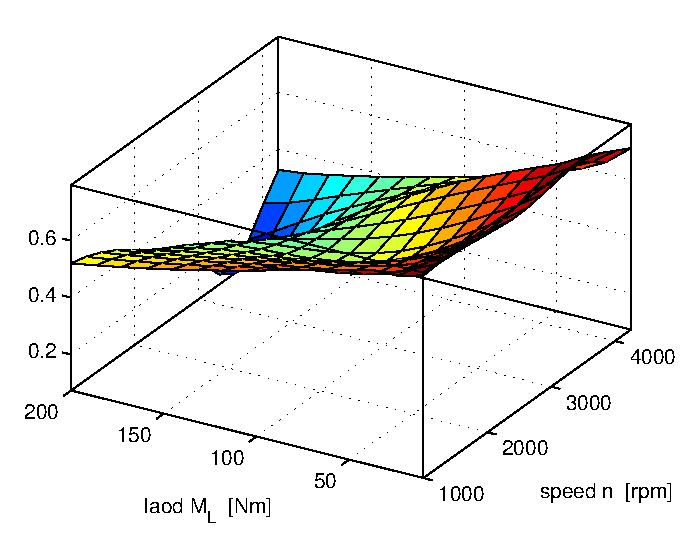
\includegraphics[width=0.75\textwidth]{img/k_surf.eps}
   \caption{Example of a figure.}
   \label{img:k_surf}
\end{figure}
\end{verbatim}

\begin{figure}[ht]
   \centering
   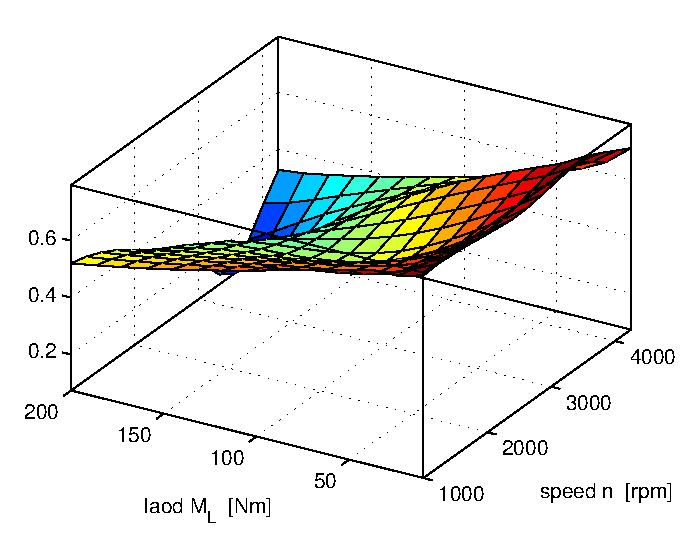
\includegraphics[width=0.75\textwidth]{img/k_surf.eps}
   \caption{Example of a figure.}
   \label{img:k_surf}
\end{figure}

Two figures are displayed next to each other using
\begin{verbatim}
\begin{figure}[ht]
  \begin{minipage}[t]{0.48\textwidth}
    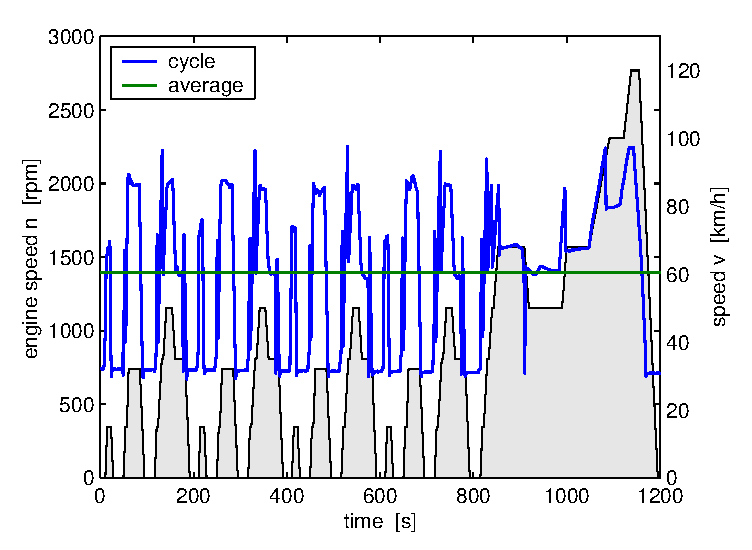
\includegraphics[width = \textwidth]{img/cycle_we.eps}
  \end{minipage}
  \hfill
  \begin{minipage}[t]{0.48\textwidth}
    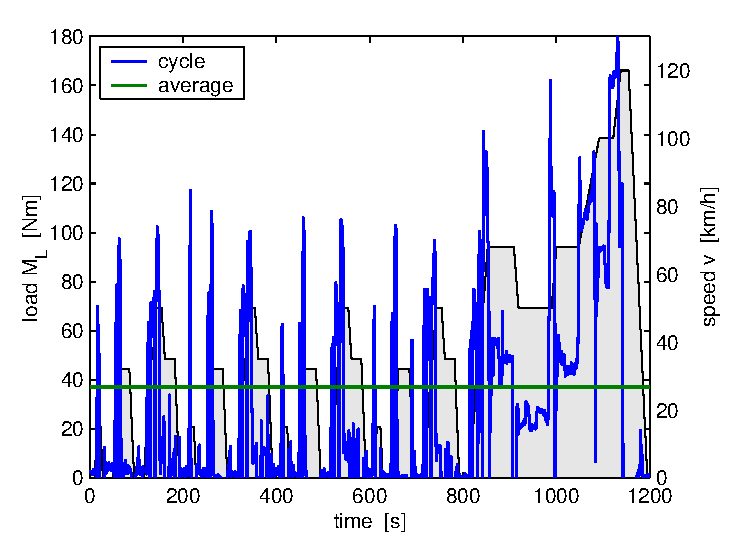
\includegraphics[width = \textwidth]{img/cycle_ml.eps}
  \end{minipage}
  \caption{Two figures next to each other.}
  \label{img:cycle}
\end{figure}
\end{verbatim}

\begin{figure}[ht]
  \begin{minipage}[t]{0.48\textwidth}
    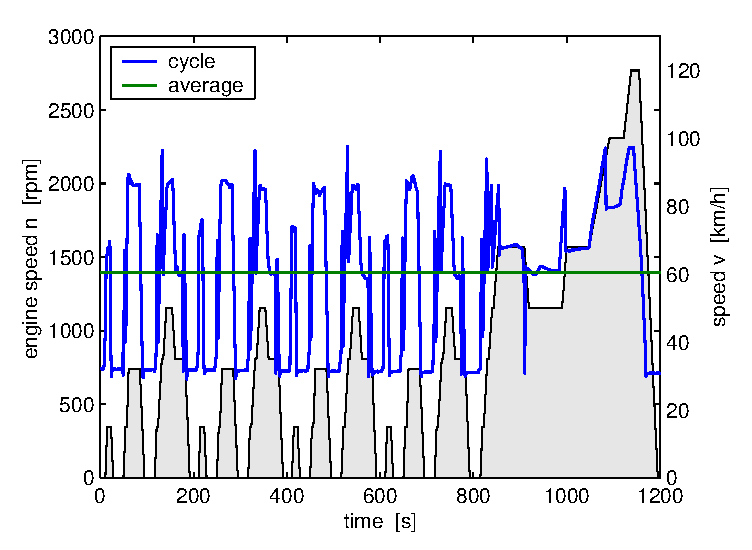
\includegraphics[width = \textwidth]{img/cycle_we.eps}
  \end{minipage}
  \hfill
  \begin{minipage}[t]{0.48\textwidth}
    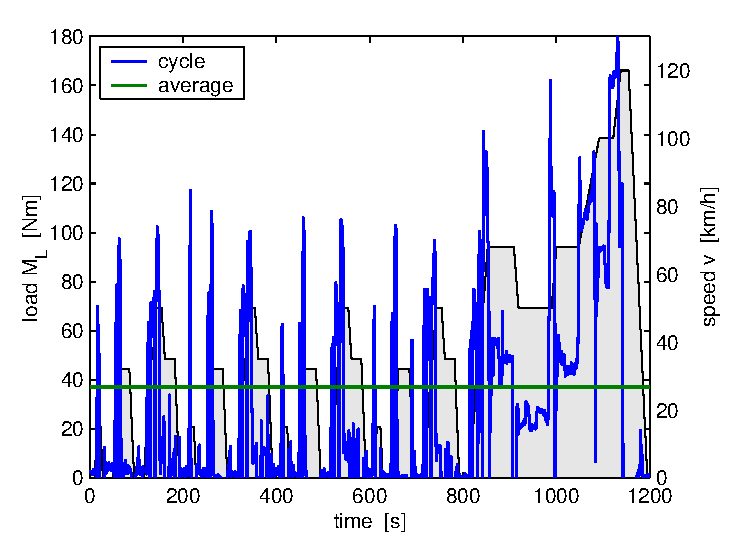
\includegraphics[width = \textwidth]{img/cycle_ml.eps}
  \end{minipage}
  \caption{Two figures next to each other.}
  \label{img:cycle}
\end{figure}

The positioning parameter \texttt{h} (here) forces your figure to be placed in the current position relative to your text. You may add \texttt{t} (top), \texttt{b} (bottom), and/or \texttt{p} (page) to allow for more flexible positioning within your document. For instance, \texttt{[tb]} forces your figure to be placed either on the top or bottom of a page.


\section{Equations}\label{sec:math}
The most common way to include equations is using the \texttt{equation} environment.
\begin{equation}\label{eq:p_me0f}
 p_\mathrm{me0f}(T_e,\omega_e) \ = \ k_1(T_e) \cdot (k_2+k_3 S^2
 \omega_e^2) \cdot \Pi_\mathrm{max} \cdot \sqrt{\frac{k_4}{B}} \, .
\end{equation}
It is recommended to use \texttt{\textbackslash mathrm\{.\}} for subscripts comprising more than two letters since it reduces the width of the subscript significantly and improves readability. The corresponding code is
\begin{verbatim}
\begin{equation}\label{eq:p_me0f}
 p_\mathrm{me0f}(T_e,\omega_e) \ = \ k_1(T_e) \cdot (k_2+k_3 S^2
 \omega_e^2) \cdot \Pi_\mathrm{max} \cdot \sqrt{\frac{k_4}{B}} \, .
\end{equation}
\end{verbatim}
Equations, such as Eq.~\eqref{eq:p_me0f}, may be referenced using \texttt{\textbackslash eqref\{.\}}. In-line mathematical content is created using \texttt{\$.\$}, for example $a^2+b^2=c^2$. It is practically possible to typeset any equation in \LaTeX. Equation~\eqref{eq:advanced} shows an example of a more advance structure.
\begin{equation}\label{eq:advanced}
x^k_n(i) = \left\{\begin{array}{ll}y(i) & \text{if}\quad x^k_{n-1}(i)\leq \mathbf{x}\\
z(i) & \text{otherwise}\end{array}\right., \text{for}\quad i=\{1,\ldots,N\}.
\end{equation}



\section{Including Code in your Document}
Include samples from your Matlab code using the \texttt{lstlistings} environment, for example
\lstset{language=Matlab,numbers=none}
\begin{lstlisting}[frame=lines]
% Evaluate y = 2x
for i = 1:length(x)

  y(i) = 2*x(i);

end
\end{lstlisting}
This example was created using
\begin{verbatim}
\lstset{language=Matlab,numbers=none}
\begin{lstlisting}[frame=lines]
% Evaluate y = 2x
for i = 1:length(x)

  y(i) = 2*x(i);

end
\end{lstlisting}
\end{verbatim}
where \texttt{\textbackslash usepackage\{mcode\}} must be included in the preamble of your document. If you want to include the entire content of a file \texttt{mycode.m} in your document, simply input the path to \texttt{mycode.m} instead of pasting the entire content into your \TeX -file
\begin{verbatim}
\lstset{language=Matlab,numbers=left}
\lstinputlisting{path/to/mycode.m}
\end{verbatim}
Including the path to your m-file also ensures that the code in your report is always up-to-date. The \texttt{\textbackslash lstset\{language=Matlab\}} command ensures that \textsc{Matlab} syntax definitions are used, but many other languages are recognised as well such as \texttt{Fortran} and \texttt{C++}.

%\cleardoublepage
% \input{}
% \cleardoublepage
% \input{}
% \cleardoublepage
% ...

% Appendix______________________________________________________________________
%\appendix
%\chapter{Quantum state preparation with Gaussian distributions}\label{sec:stateprepgaussian}

To keep the discussion simple, the task is to load one Gaussian input distribution $R$ and two Gaussian training samples, $L_1$ and $L_2$, such that the amplitude-based kNN algorithm can be used to classify $R$. Note that the input and training distributions are restricted to Gaussian distributions that can be initialized by using the coin gate $C(\delta)$ for some value of $\delta$. The input and training samples all have $N$ entries whereby $N$ is restricted to be a multiple of two. To encode the distributions, $n$ data qubits are required such that there are $2^n = N$ amplitudes. Additionally, one ancilla, one class and one $m$ qubit are needed. Since all qubits are initialised to the \0 state, the initial state is 

\begin{equation}
\ket{\Upsilon_0} = \ket{a;d_1,...,d_n;c;m} = \ket{0;0_1,...,0_n;0;0}
\end{equation}

where the first register holds the ancilla ($a$), the second register holds the $n$ data qubits ($d$) used to encode the distributions and the third and fourth register consists of the class ($c$) and $m$-qubit respectively.

As already demonstrated in Eq.~\ref{equ:chi1} and Eq.~\ref{equ:chi2} in Section~\ref{subsubsec:implementationamplitudeKNN}, the ancilla and $m$-register are each put into an equal superposition through the application of two H gates. The state is then

\begin{equation}
\ket{\Upsilon_1} = \frac{1}{2} \sum_{m=0}^1 \big[ \ket{0}\ket{0_1,...,0_n} + \ket{1}\ket{0_1,...,0_n}\big] \ket{0}\ket{m}
\end{equation}

Suppose the Gaussian distribution $R$ is obtained by choosing $\delta = \tau$ for the coin gate $C(\delta)$. Then the next step is to make use of the controlled version of the coin gate $CC(\tau)$ controlled by the ancilla qubit. $CC(\tau)$ is applied to each of the $n$ qubits in the data register to load the input distribution $R$. Hence, the new quantum state is 

\begin{equation}
\ket{\Upsilon_2} = \prod^n_{j=1} CC(\tau)(a,d_j) \ket{\Upsilon_1} = \frac{1}{2} \sum_{m=0}^1 \big[ \ket{0}\ket{0_1,...,0_n} + \ket{1}\ket{R}\big] \ket{0}\ket{m}
\end{equation}

Since the algorithm is simulated in Liqui$\ket{}$, it is straightforward to define the controlled version of the coin gate $C(\delta)$. 

Next, using an X gate to flip the ancilla moves the input distribution $R$ onto the \0 state of the ancilla such that the state is now

\begin{equation}
\ket{\Upsilon_3} = X(a) \ket{\Upsilon_2} = \frac{1}{2} \sum_{m=0}^1 \big[ \ket{0}\ket{R} + \ket{1}\ket{0_1,...,0_n}\big] \ket{0}\ket{m}
\end{equation}

Suppose the first training distribution $L_1$ can be loaded by choosing $\delta = \sigma$ and applying $C(\sigma)$ to the qubit pattern $\ket{0_1,...,1_5,0_6,...,0_n}$. Thus, the fifth qubit in the data register connected to the \1 ancilla state needs to flipped into the \1 state. This can be done with a CCNOT gate, controlled by the ancilla and $m$ qubit, acting on the fifth data qubit. Next, by applying the controlled controlled version of the coin gate $CCC(\sigma)$ to each data qubit controlled by the ancilla and the $m$ qubit the training sample $L_1$ is loaded. The quantum state is then given by
\begin{align}
\ket{\Upsilon_4} &= \prod^n_{j=1} CCC(\sigma)(a,m,d_j) CCNOT(a,m,d_5) \ket{\Upsilon_3}\notag\\
&= \frac{1}{2} \Big[\big[ \ket{0}\ket{R} + \ket{1}\ket{0_1,...,0_n}\big] \ket{0}\ket{0} + \big[\ket{0}\ket{R} + \ket{1}\ket{L_1*}\big] \ket{0}\ket{1}\Big]
\end{align}

Since the last entry on the diagonal of the coin gate (see Eq.~\ref{equ:coingate}) is negative, the application of $CCC(\sigma)$ introduces a negative sign when applied to the fifth data qubit. Hence, not the exact distribution $L_1$ but a distribution $L_1^*$ with a sign difference was loaded into $\ket{\Upsilon_4}$. As explained in Section~\ref{subsec:amplitudeKNNalgorithm}, the amplitude-based kNN algorithm makes use of interference between the input and training samples whereby the negative sign would alter the outcome of the interference. Thus, the sign needs to be corrected by acting a controlled controlled Z gate on the fifth data qubit. Thereafter, the $m$ qubit is flipped with an X gate to move $L_1$ onto the \0 state of the $m$ qubit. After these gate operations the state is
\begin{align}
\ket{\Upsilon_5} &= X(m) CCZ(d_5) \ket{\Upsilon_4}\notag\\
&= \frac{1}{2} \Big[\big[ \ket{0}\ket{R} + \ket{1}\ket{L_1}\big] \ket{0}\ket{0} + \big[\ket{0}\ket{R} + \ket{1}\ket{0_1,...,0_n}\big] \ket{0}\ket{1}\Big]
\end{align}

For the second training distribution $L_2$, suppose it results from choosing $\delta = \nu$ and applying $C(\nu)$ to the qubit pattern $\ket{1_1,...,1_n}$. Thus, all data qubits connected to the \1 ancilla and \1 $m$-qubit state have to be flipped using a CCNOT gates. As outlined in the previous step, $CCC(\nu)$ loads the distribution $L_2^*$ and not $L_2$ because of sign differences. Since all data qubits are \1, these signs are corrected by acting controlled controlled Z gates on all data qubits controlled by the ancilla and $m$-qubit. The state containing the input and both training distributions is then

\begin{align}
\ket{\Upsilon_6} &= \prod^n_{j=1} CCZ(d_j) CCC(\sigma)(a,m,d_j) CCNOT(a,m,d_j) \ket{\Upsilon_5}\notag\\
&= \frac{1}{2} \Big[\big[ \ket{0}\ket{R} + \ket{1}\ket{L_1}\big] \ket{0}\ket{0} + \big[\ket{0}\ket{R} + \ket{1}\ket{L_2}\big] \ket{0}\ket{1}\Big]
\end{align}

Lastly, the class qubit for $L_2$ is flipped with a CNOT gate controlled by the $m$ qubit such that the final state is
\begin{align}
\ket{\Upsilon_6} &= CNOT(m,c) \ket{\Upsilon_6}\notag\\
&= \frac{1}{2} \Big[\big[ \ket{0}\ket{R} + \ket{1}\ket{L_1}\big] \ket{0}\ket{0} + \big[\ket{0}\ket{R} + \ket{1}\ket{L_2}\big] \ket{1}\ket{1}\Big]
\end{align}


$\ket{\Upsilon_7}$ is in the form of the initial quantum state (Eq.~\ref{equ:ampinitial}) required for the amplitude-based kNN algorithm. This completes the quantum state preparation routine for loading a restricted subset of discrete Gaussian distributions using the coin gate $C(\delta)$.

 \cleardoublepage



% Bibliography__________________________________________________________________
% Literature (Additional references can be added to the .bib-file manually, or by using, for example, the free application JabRef). Compile in the following order: latex -bibtex -latex -latex

\bibliographystyle{apacite}
\bibliography{thesis}

\end{document}
